\begin{figure}[htp]
	\centering
	\subfloat[\(\mesh{S_{1}},\ \mu=1.00\)]
	{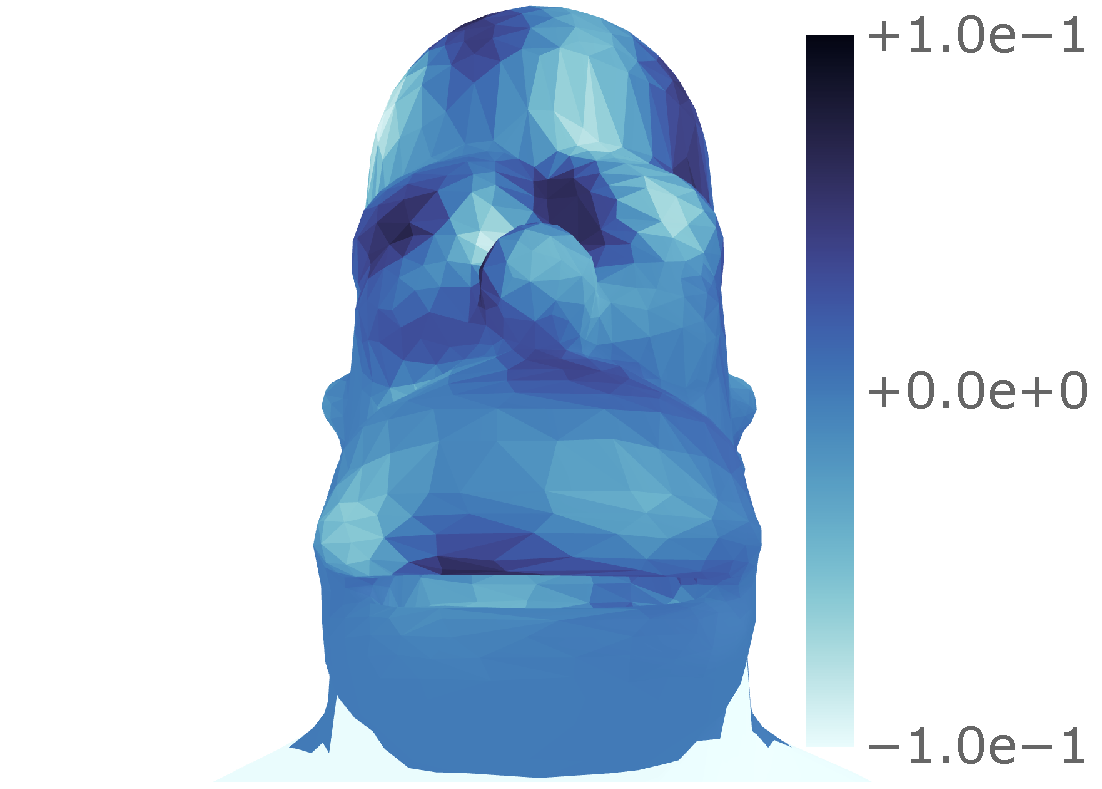
\includegraphics[trim={102 3 6 2},clip,width=.33\textwidth]{chapter4/slepian_homer_rank0_lam1-000000e00_zoom.pdf}} % chktex 8
	\hfill
	\subfloat[\(\mesh{S_{10}},\ \mu=1.00\)]
	{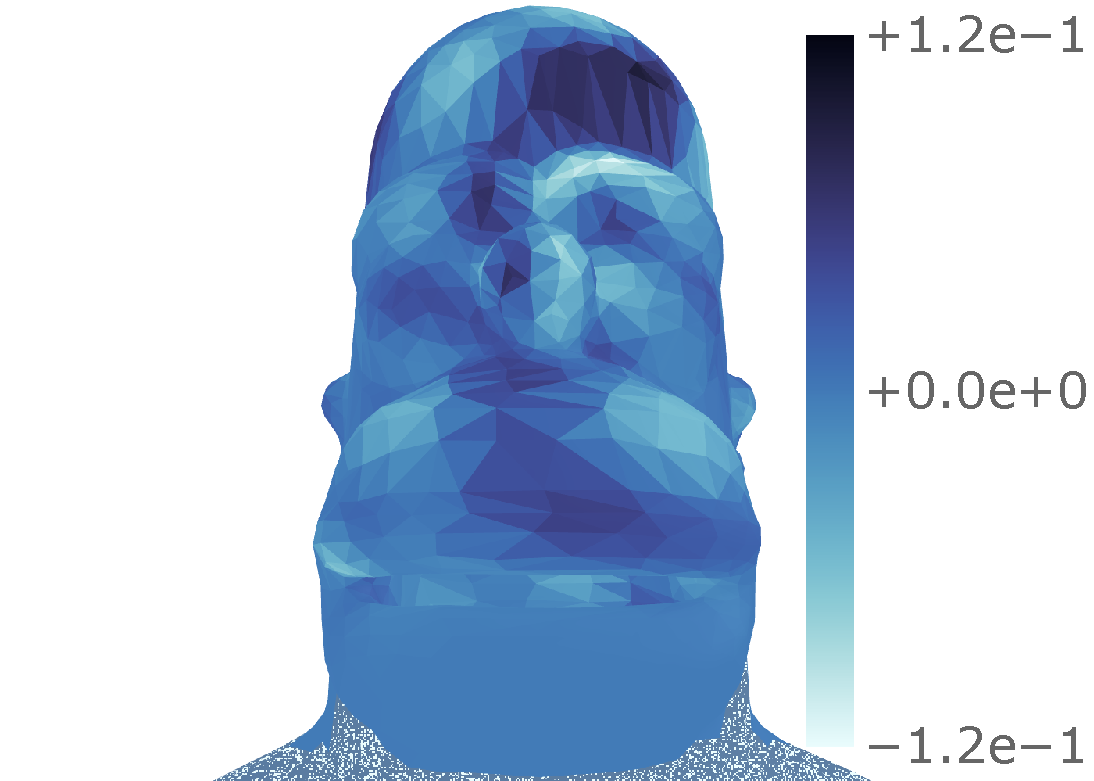
\includegraphics[trim={102 3 6 2},clip,width=.33\textwidth]{chapter4/slepian_homer_rank9_lam1-000000e00_zoom.pdf}} % chktex 8
	\hfill
	\subfloat[\(\mesh{S_{25}},\ \mu=1.00\)]
	{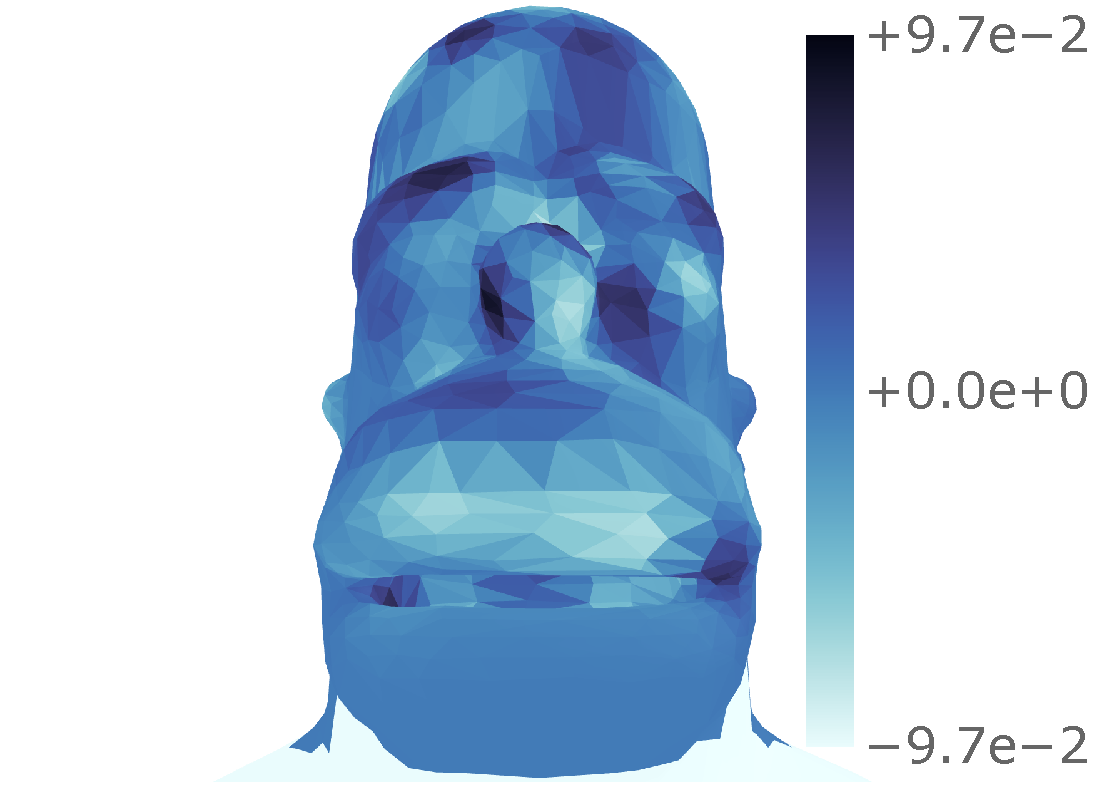
\includegraphics[trim={102 3 6 2},clip,width=.33\textwidth]{chapter4/slepian_homer_rank24_lam1-000000e00_zoom.pdf}} % chktex 8
	\newline
	\subfloat[\(\mesh{S_{50}},\ \mu=1.00\)]
	{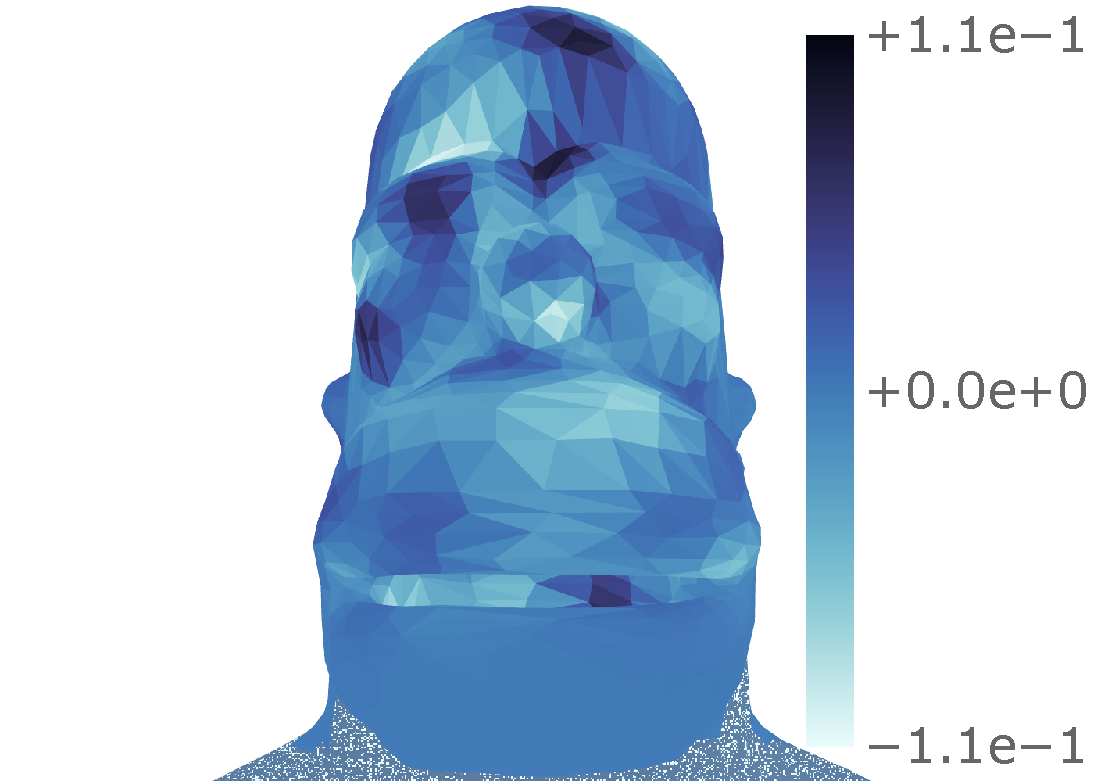
\includegraphics[trim={102 3 6 2},clip,width=.33\textwidth]{chapter4/slepian_homer_rank49_lam1-000000e00_zoom.pdf}} % chktex 8
	\hfill
	\subfloat[\(\mesh{S_{100}},\ \mu=1.00\)]
	{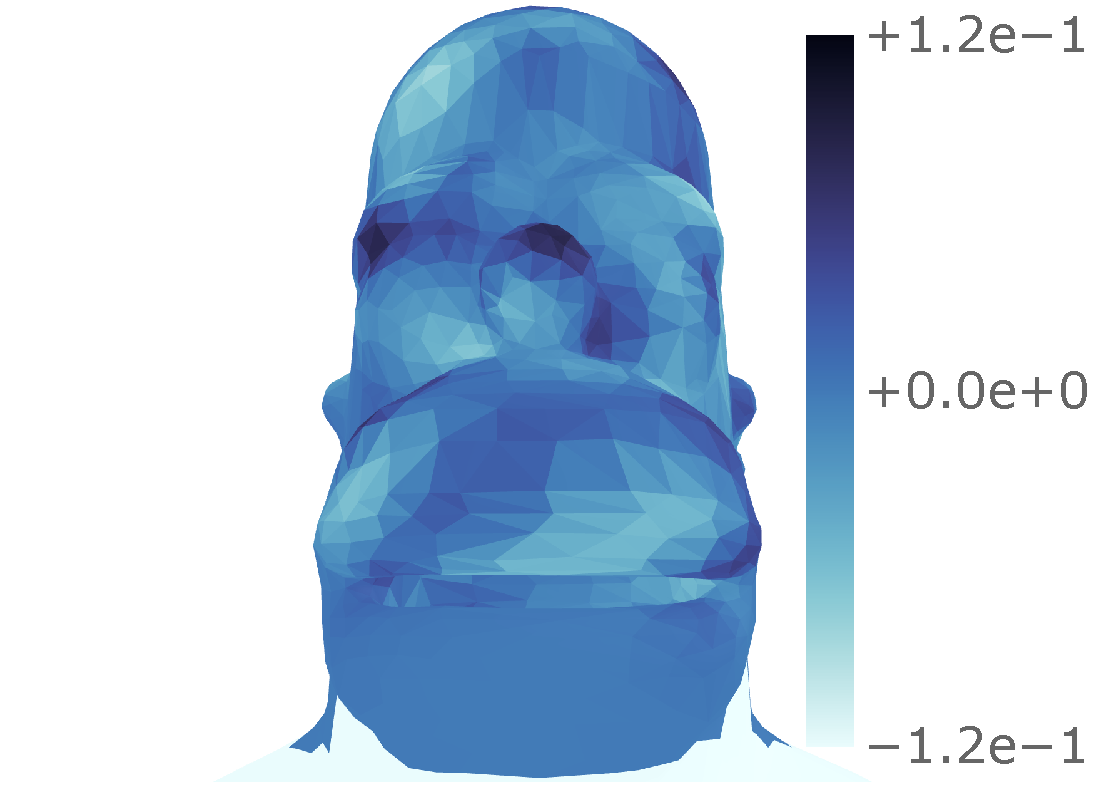
\includegraphics[trim={102 3 6 2},clip,width=.33\textwidth]{chapter4/slepian_homer_rank99_lam1-000000e00_zoom.pdf}} % chktex 8
	\hfill
	\subfloat[\(\mesh{S_{200}},\ \mu=1.00\)]
	{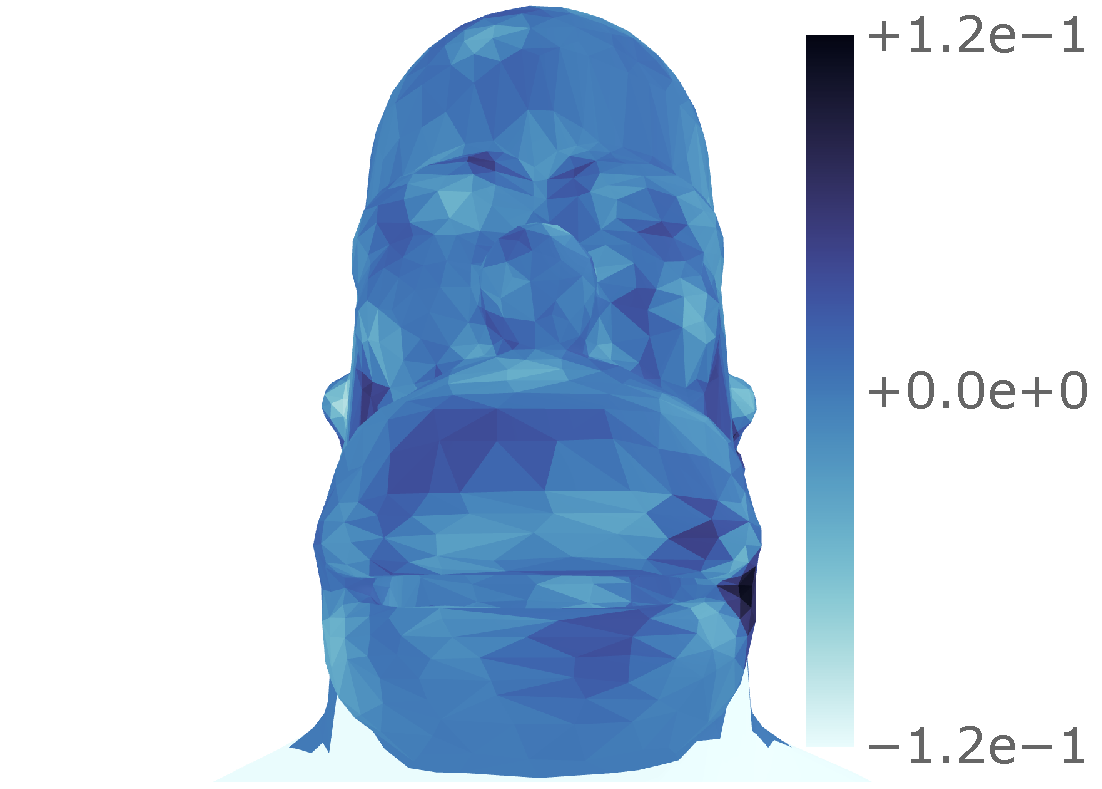
\includegraphics[trim={102 3 6 2},clip,width=.33\textwidth]{chapter4/slepian_homer_rank199_lam1-000000e00_zoom.pdf}} % chktex 8
	\caption{
	}\label{fig:chapter4_slepian_functions}
\end{figure}
